\subsubsection{Numerische Lösungsverfahren}

Der kontinuierliche Modellansatz führt zu Feldgleichungen in Form von partiellen Differentialgleichungen. Anwendungsgebiete sind hier die Strukturmechanik, der Stoff- und Wärmetransport sowie die Elektrostatik und viele weitere Bereiche. Diese partiellen Differentialgleichungen können in der Regel nicht analytisch gelöst werden, weshalb sich numerische Berechnungsschemata hierfür etabliert haben. Die heute gebräuchlichsten werden im Folgenden kurz beschrieben:

\begin{itemize}
\item Netzbasierte Methoden:\begin{itemize}
\item Finite-Elemente-Methode \textbf{(FEM)}
\item Finite-Volumen-Methode \textbf{(FVM)}
\item Finite-Differenzen-Methode \textbf{(FDM)}
\item Randelementmethode \textbf{(BEM)}
\item Discontinuous Galerkin Methods \textbf{(DG)}
\end{itemize}


\item Netzunabhängige Methoden:\begin{itemize}
\item Optimal Transport Method \textbf{(OTM)}
\item Element-Free Galerkin \textbf{(EFG)}
\item Moving Least Squares \textbf{(MLS)}
\end{itemize}


\item Kombination:\begin{itemize}
\item Material Point Method \textbf{(MPM)}
\end{itemize}


\item ...
\end{itemize}

Alle diese Methoden haben eine Gemeinsamkeit: Sie führen auf ein Gleichungssystem der Form:
\begin{equation}
\label{LGS}
\boldsymbol{Ax}=\boldsymbol{b}
\end{equation}
mit der Systemmatrix $\boldsymbol{A}$. Im Folgenden soll nur kurz auf die 4 am weitesten verbreiteten Methoden eingegangen werden.

%  -+-+-+-+-+-+-AI-SPLIT

\paragraph{Finite Differenzen Methode (FDM)}

Die Finite Differenzen Methode (FDM) ist ein numerisches Verfahren zur Lösung partieller Differentialgleichungen (PDEs), das auf der Approximation der Ableitungen durch Differenzenquotienten basiert. Hier sind die grundlegenden Schritte und Konzepte der FDM:

\begin{enumerate}
\item \textbf{Diskretisierung des Raums}: Der kontinuierliche Raum wird in ein Gitter unterteilt. Die Punkte auf diesem Gitter werden als Gitterpunkte bezeichnet.
\item \textbf{Approximation der Ableitungen}: Die Ableitungen in der PDE werden durch finite Differenzen approximiert. Zum Beispiel kann die erste Ableitung einer Funktion $u$ an einem Punkt $i$ durch den zentralen Differenzenquotienten approximiert werden:
\end{enumerate}
\begin{equation}
\frac{du}{dx} \approx \frac{u_{i+1} - u_{i-1}}{2\Delta x}
\end{equation}
oder durch den vorwärts gerichteten Differenzenquotienten:
\begin{equation}
\frac{du}{dx} \approx \frac{u_{i+1} - u_i}{\Delta x}
\end{equation}
\begin{enumerate}[resume]
\item \textbf{Aufstellen eines Gleichungssystems}: Durch das Einsetzen der approximierten Ableitungen in die ursprüngliche PDE wird ein System von algebraischen Gleichungen aufgestellt, das die Werte der Funktion an den Gitterpunkten beschreibt.
\item \textbf{Lösen des Gleichungssystems}: Das resultierende Gleichungssystem kann mit verschiedenen numerischen Verfahren gelöst werden.
\end{enumerate}

Die Finite Differenzen Methode ist einfach zu implementieren und eignet sich gut für Probleme mit regelmä$\beta$igen Gitterstrukturen. Sie hat jedoch Einschränkungen bei der Behandlung komplexer Geometrien und kann in der Nähe von Randbedingungen oder Singularitäten weniger genau sein.

%  -+-+-+-+-+-+-AI-SPLIT

\paragraph{Finite Volumen Methode (FVM)}

Die Finite Volumen Methode  ist ein numerisches Verfahren zur Lösung partieller Differentialgleichungen (PDEs), das insbesondere in der Strömungsmechanik und bei der Simulation von Transportphänomenen weit verbreitet ist. Hier sind die grundlegenden Schritte und Konzepte der FVM:

\begin{enumerate}
\item \textbf{Diskretisierung des Raums}: Der kontinuierliche Raum wird in eine endliche Anzahl von Kontrollvolumen unterteilt. Jedes Kontrollvolumen ist ein kleines Volumen, das um einen Gitterpunkt zentriert ist. Diese Volumina können regelmä$\beta$ig oder unregelmä$\beta$ig sein, je nach der Geometrie des Problems.
\item \textbf{Integralform der PDE und Flussdiskretisierung}: Die PDE wird in ihrer Integralform formuliert und über jedes Kontrollvolumen integriert. Durch Anwendung des Gauss'schen Integralsatzes wird die Integralform in eine Form umgewandelt, die die Flüsse an den Grenzen der Kontrollvolumen berücksichtigt. Die Flüsse an den Grenzen werden approximiert, häufig durch Mittelwerte der Variablen an den benachbarten Kontrollvolumen oder durch spezielle Interpolationsmethoden.
\item \textbf{Aufstellen eines Gleichungssystems}: Durch die Diskretisierung der Flüsse und das Einsetzen in die Integralform wird ein System von algebraischen Gleichungen aufgestellt, das die Werte der gesuchten Variablen an den Gitterpunkten beschreibt.
\item \textbf{Lösen des Gleichungssystems}: Das resultierende Gleichungssystem kann mit verschiedenen numerischen Verfahren gelöst werden.
\end{enumerate}

Die Finite Volumen Methode ist besonders vorteilhaft, da sie die Erhaltungsgesetze direkt in die Berechnungen integriert und somit eine physikalisch konsistente Lösung gewährleistet. Sie eignet sich gut für Probleme mit komplexen Geometrien und ist robust gegenüber nichtlinearen Effekten. FVM wird häufig in der Strömungsmechanik, Wärmeübertragung und anderen Bereichen eingesetzt, in denen der Transport von Stoffen oder Energie eine Rolle spielt.

%  -+-+-+-+-+-+-AI-SPLIT

\paragraph{Randelemente Methode (BEM)}

Die Randelemente Methode (BEM) ist ein numerisches Verfahren zur Lösung partieller Differentialgleichungen (PDEs), das sich auf die Randbedingungen des Problems konzentriert. Hier sind die grundlegenden Schritte und Konzepte der BEM:

\begin{enumerate}
\item \textbf{Reduktion des Problems auf den Rand}: Anstatt das gesamte Volumen des Problems zu diskretisieren, wird nur der Rand des betrachteten Gebiets in Betracht gezogen. Dies reduziert die Dimension des Problems, da nur die Randflächen (2D) oder Randlinien (1D) diskretisiert werden müssen.
\item \textbf{Formulierung der Integralgleichungen}: Die PDE wird in eine Integralform umgewandelt, die die Randbedingungen berücksichtigt. Diese Integralgleichungen beschreiben die Beziehung zwischen den Werten der gesuchten Funktion und ihren Ableitungen auf dem Rand des Gebiets.
\item \textbf{Diskretisierung des Randes}: Der Rand wird in eine endliche Anzahl von Elementen unterteilt, und die gesuchte Funktion wird durch Basisfunktionen approximiert, die auf diesen Elementen definiert sind. Dies führt zu einem System von algebraischen Gleichungen, das die Werte der gesuchten Funktion an den Randpunkten beschreibt.
\item \textbf{Lösen des Gleichungssystems}: Das resultierende Gleichungssystem kann mit verschiedenen numerischen Verfahren gelöst werden.
\end{enumerate}

Die Randelemente Methode ist besonders vorteilhaft, da sie die Dimension des Problems reduziert und somit die Anzahl der benötigten Berechnungen verringert. Sie ist besonders effektiv für Probleme mit unendlichen oder halbunendlichen Domänen, wie z.B. in der Elastizitätstheorie oder der Akustik. BEM ist jedoch oft auf Probleme mit linearen PDEs und gut definierten Randbedingungen beschränkt. Das hei$\beta$t, materielle Nichtlinearitäten können nicht berücksichtigt werden (keine Plastizität!).

%  -+-+-+-+-+-+-AI-SPLIT

\paragraph{Finite Elemente Methode (FEM)}

Die Finite-Elemente-Methode (FEM) ist ein weit verbreitetes numerisches Verfahren zur Lösung partieller Differentialgleichungen (PDEs), das insbesondere in der Ingenieurwissenschaft und der Physik Anwendung findet. Hier sind die grundlegenden Schritte und Konzepte der FEM:

\begin{enumerate}
\item \textbf{Diskretisierung des Gebiets}: Der kontinuierliche Raum wird in eine endliche Anzahl von kleinen, nicht überlappenden Elementen unterteilt, die zusammen ein Netz (Mesh) bilden. Diese Elemente können verschiedene Formen haben, wie Dreiecke, Vierecke (in 2D) oder Tetraeder, Hexaeder (in 3D).
\item \textbf{Aufstellen der Elementgleichungen}: Für jedes Element wird eine lokale Formulierung der PDE aufgestellt, die die physikalischen Gesetze und Randbedingungen berücksichtigt. Dies geschieht häufig durch die Anwendung des Prinzips der virtuellen Verrückungen oder der Galerkin-Methode, um die Differentialgleichung in eine schwache Form zu überführen.
\item \textbf{Zusammenfügen der Elementgleichungen}: Die lokalen Gleichungen der einzelnen Elemente werden zu einem globalen Gleichungssystem zusammengefügt. Dies geschieht unter Berücksichtigung der Koppelung zwischen benachbarten Elementen und der gemeinsamen Knotenpunkte.
\item \textbf{Lösen des Gleichungssystems}: Das resultierende globale Gleichungssystem wird mit numerischen Verfahren gelöst.
\end{enumerate}

Die Finite-Elemente-Methode ist besonders vorteilhaft, da sie komplexe Geometrien und Materialverhalten effizient behandeln kann. Sie ermöglicht die Analyse von statischen und dynamischen Problemen in verschiedenen Bereichen, wie Strukturmechanik, Wärmeübertragung und Fluiddynamik. FEM ist flexibel und anpassungsfähig, erfordert jedoch eine sorgfältige Netzgenerierung und kann bei sehr feinen Netzen rechenintensiv sein.

%  -+-+-+-+-+-+-AI-SPLIT

\paragraph{Zusammenfassung}

\begin{figure}[!htbp]
\centering
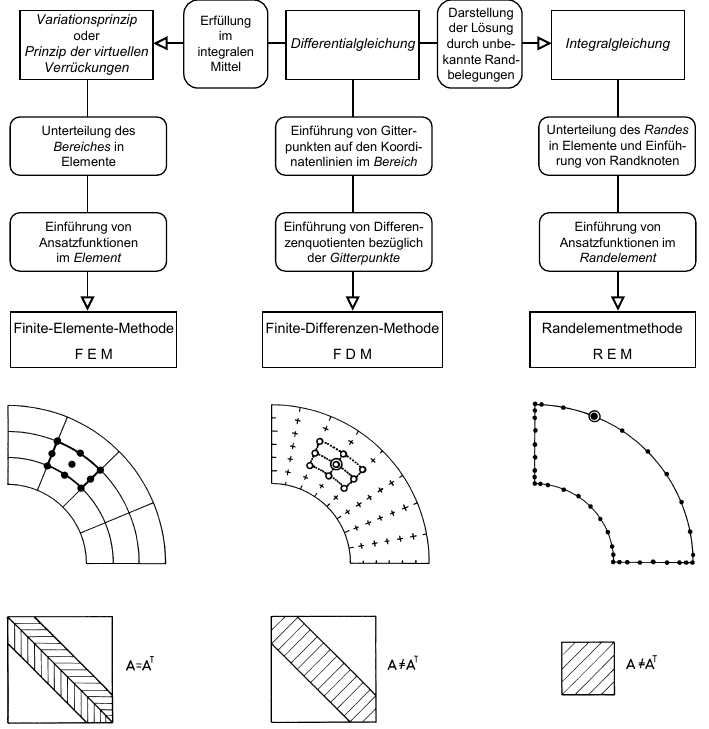
\includegraphics[width=0.7\linewidth]{files/Diskretisierungsverf-3291ac8fb462ef44b4d348533f5b41ac.png}
\caption[]{Vergleich verschiedener Diskretisierungsverfahren nach \cite{knothe1991finite}}
\label{diskretisierungsvergleich}
\end{figure}

Jede der oben genannten Methoden hat ihre Daseinsberechtigung für gewählte Problemstellungen. Für die Strukturmechanik hat sich die Finite-Elemente-Methode durchgesetzt, da sie am flexibelsten und effizientesten eingesetzt werden kann. Dies wird in Abbildung Figure~\ref{diskretisierungsvergleich} deutlich. Die resultierende Systemmatrix $A$ ist für viele Problemstellungen symmetrisch und weist eine ausgesprochene Bandstruktur auf, was für die Lösung des Gleichungssystems erhebliche Vorteile bringt.

\bigskip\noindent
\begin{tabular}{p{\dimexpr 0.200\linewidth-2\tabcolsep}p{\dimexpr 0.200\linewidth-2\tabcolsep}p{\dimexpr 0.200\linewidth-2\tabcolsep}p{\dimexpr 0.200\linewidth-2\tabcolsep}p{\dimexpr 0.200\linewidth-2\tabcolsep}}
\toprule
Methode & Dimension & Ansatz & Vorteile & Nachteile \\
\hline
\textbf{FEM} & Volumen & Diskretisierung des gesamten Gebiets in Elemente & Flexibel für komplexe Geometrien und Materialverhalten; gut für statische und dynamische Probleme & Erfordert sorgfältige Netzgenerierung; rechenintensiv bei feinen Netzen \\
\textbf{BEM} & Rand & Reduktion des Problems auf den Rand des Gebiets & Reduziert die Dimension des Problems; effizient bei unendlichen oder halbunendlichen Domänen & Beschränkt auf Probleme mit gut definierten Randbedingungen; oft nur für lineare PDEs geeignet \\
\textbf{FDM} & Volumen & Diskretisierung des Gebiets in Gitterpunkte & Einfach zu implementieren; gut für regelmä$\beta$ige Geometrien & Schwierigkeiten bei komplexen Geometrien; weniger genau in der Nähe von Singularitäten \\
\textbf{FVM} & Volumen & Diskretisierung des Gebiets in Kontrollvolumen & Berücksichtigt Erhaltungsgesetze direkt; robust bei nichtlinearen Effekten & Kann komplexer in der Implementierung sein; erfordert sorgfältige Flussapproximation \\
\bottomrule
\end{tabular}

\bigskip Jede Methode hat ihre eigenen Stärken und Schwächen, und die Wahl der Methode hängt oft von der spezifischen Anwendung ab.

%  -+-+-+-+-+-+-AI-SPLIT

\begin{framed}
\textbf{Fragen zum Kapitel}\\
\textbf{Numerische Lösungsverfahren}

\begin{itemize}
\item Nennen Sie drei Verfahren zur Lösung von partiellen Differentialgleichungen (Feldgleichungen).
\item Warum benötigen wir numerische Verfahren zur Lösung der Feldgleichungen?
\item In allen numerischen Verfahren werden die Feldgleichungen umgeformt. Was muss letztendlich bei allen Verfahren gelöst werden?
\item Welches numerische Verfahren ist besonders gut für Strömungsprobleme geeignet?
\item Nennen Sie drei Gründe, warum sich die FEM in der Strukturmechanik durchgesetzt hat?
\end{itemize}
\end{framed}